\documentclass[11pt, letterpaper, twocolumn]{article}

% Packages
\usepackage[utf8]{inputenc}
\usepackage[T1]{fontenc}
\usepackage[margin=1in]{geometry}
\usepackage{cite}
\usepackage{amsmath}
\usepackage{graphicx}
\usepackage{url}
\usepackage{hyperref}
\usepackage{listings}
\usepackage{xcolor}
\usepackage{booktabs}
\usepackage{tabularx}
\usepackage{enumitem}
\usepackage{tikz}
\usetikzlibrary{arrows.meta, positioning, shapes.geometric, fit, calc}
% Page numbers
\pagestyle{plain}

% Hyperref configuration
\hypersetup{
    colorlinks=true,
    linkcolor=blue!70!black,
    citecolor=blue!70!black,
    urlcolor=blue!70!black,
}

% Code listing style
\lstdefinestyle{powershell}{
    backgroundcolor=\color{gray!10},
    basicstyle=\ttfamily\footnotesize,
    breaklines=true,
    frame=single,
    rulecolor=\color{gray!40},
    numbers=left,
    numberstyle=\tiny\color{gray},
    keywordstyle=\color{blue!70!black}\bfseries,
    commentstyle=\color{green!50!black}\itshape,
    stringstyle=\color{red!70!black},
    showstringspaces=false,
    tabsize=4,
    captionpos=b,
}

\lstdefinestyle{json}{
    backgroundcolor=\color{gray!10},
    basicstyle=\ttfamily\footnotesize,
    breaklines=true,
    frame=single,
    rulecolor=\color{gray!40},
    numbers=left,
    numberstyle=\tiny\color{gray},
    showstringspaces=false,
    tabsize=2,
    captionpos=b,
}

\lstset{style=powershell}

% Title
\title{AI-Assisted Development for Government Compliance:\\Using Claude Code to Meet Federal Information Security Requirements}

\author{
    Bruce Dombrowski\\
    \textit{Independent Researcher}\\
    \small GitHub: brucedombrowski
}

\begin{document}

\maketitle

% ============================================================
\begin{abstract}
Government software development demands rigorous compliance with federal standards including NIST Special Publications, FIPS cryptographic requirements, and CUI handling regulations under 32~CFR~Part~2002. These requirements impose significant documentation overhead---formal requirements traceability, decision memoranda, verification matrices, and regulatory cross-references---that traditionally consumes substantial engineering effort. This paper examines the application of Claude Code, Anthropic's AI-powered command-line development tool, to government compliance software projects. Drawing on three real-world case studies---a CUI email encryption tool (SendCUIEmail), a formal decision documentation system, and a Security Verification Toolkit implementing automated NIST SP 800-53 control verification---we demonstrate how AI-assisted development can accelerate compliance artifact generation while maintaining the precision required by federal auditors. We present a five-phase methodology for structuring AI agent workflows around government documentation standards---from requirements capture through version-controlled interaction traceability using git and GitHub issues---evaluate the quality of AI-generated compliance artifacts against manual baselines, and discuss the implications for federal software development practices. Our findings suggest that AI-assisted tooling can reduce compliance documentation effort by shifting the engineer's role from author to reviewer, while the interactive agent model provides the human-in-the-loop oversight that government frameworks require.
\end{abstract}

\medskip
\noindent\textbf{Keywords:} AI-assisted development, government compliance, NIST, FIPS, CUI, controlled unclassified information, Claude Code, large language models, software engineering, federal information security

% ============================================================
\section{Introduction}
\label{sec:introduction}

Federal information security requirements impose a dual burden on software developers: the software must correctly implement cryptographic and handling standards, and the \textit{process} of building that software must be formally documented. A tool that encrypts files per FIPS~197 \cite{fips197} is insufficient if the development team cannot produce a requirements traceability matrix linking each implementation decision to the governing standard. This documentation overhead---decision memoranda, verification documents, requirements specifications---is where many small teams and independent developers struggle to meet government expectations.

The emergence of AI-powered development tools offers a potential path forward. Large language models (LLMs) trained on technical and regulatory corpora can draft compliance documents, suggest standard references, and generate structured artifacts. However, government work demands accuracy: an incorrect citation to a NIST Special Publication or a mischaracterized FIPS requirement could undermine an entire compliance package.

Claude Code, Anthropic's command-line interface for the Claude family of models, provides an interactive development environment where the AI agent operates directly within the developer's file system and terminal. Unlike web-based chat interfaces, Claude Code can read source files, execute build commands, search codebases, and write artifacts---all under explicit developer approval. This architecture maps naturally to the human-in-the-loop oversight model that government compliance frameworks expect.

This paper makes the following contributions:

\begin{enumerate}[leftmargin=*]
    \item A five-phase methodology for using AI agents in government compliance software development, from requirements capture through version-controlled interaction traceability.
    \item Three case studies demonstrating AI-assisted development of compliance artifacts: SendCUIEmail (a CUI encryption tool), a LaTeX-based decision memoranda system, and a Security Verification Toolkit implementing automated NIST SP 800-53 control verification.
    \item An audit traceability framework using git (configuration management) and GitHub issues (interaction logging) to provide bidirectional provenance between human directives and AI-generated artifacts.
    \item A standards-based review process mapped to IEEE~1028, NIST SP 800-53, and ISO/IEC~25010, with enforced separation of duties between authoring and auditing agents.
    \item A discussion of the \texttt{--agents} mode workflow for multi-agent collaboration on compliance projects.
\end{enumerate}

% ============================================================
\section{Background and Related Work}
\label{sec:background}

\subsection{Government Compliance Landscape}

Federal information security is governed by a layered framework of executive orders, regulations, and technical standards. Executive Order~13556 established the Controlled Unclassified Information (CUI) program, implemented through 32~CFR~Part~2002 \cite{32cfr2002}. The National Institute of Standards and Technology (NIST) provides the technical backbone through publications including:

\begin{itemize}[leftmargin=*]
    \item \textbf{NIST SP 800-171} \cite{nist800171}: Protecting CUI in Nonfederal Information Systems
    \item \textbf{NIST SP 800-53} \cite{nist80053}: Security and Privacy Controls for Information Systems
    \item \textbf{NIST SP 800-132} \cite{nist800132}: Recommendation for Password-Based Key Derivation
    \item \textbf{FIPS 197} \cite{fips197}: Advanced Encryption Standard (AES)
    \item \textbf{FIPS 140-2} \cite{fips1402}: Security Requirements for Cryptographic Modules
\end{itemize}

Compliance requires not only that software implementations adhere to these standards, but that organizations maintain documentation demonstrating adherence---what auditors term ``evidence of compliance.'' This evidence typically includes requirements specifications, design decisions, test plans, and verification matrices that trace each requirement to its implementation and test.

\subsection{AI-Assisted Software Development}

The application of large language models to software engineering has been studied extensively \cite{fan2023llmse}. Code generation tools such as GitHub Copilot, Amazon CodeWhisperer, and Anthropic's Claude have demonstrated capability in producing syntactically correct code across multiple languages. However, the application of LLMs to \textit{compliance-oriented} development---where correctness encompasses not just functional behavior but regulatory adherence---remains underexplored.

Prior work on AI-assisted documentation generation has focused primarily on API documentation \cite{khan2022apidoc} and code comments. The generation of \textit{regulatory} documentation---where the AI must reason about the relationship between code implementations and published standards---presents distinct challenges including citation accuracy, regulatory interpretation, and the need for conservative (rather than creative) text generation.

\subsection{Claude Code Architecture}

Claude Code operates as a command-line agent with access to the developer's local environment. Key architectural properties relevant to compliance work include:

\begin{enumerate}[leftmargin=*]
    \item \textbf{File system access}: The agent reads and writes files directly, enabling it to analyze source code and produce artifacts in-place.
    \item \textbf{Tool use with approval}: Each action (file read, edit, command execution) requires developer approval, providing the human oversight that compliance frameworks demand.
    \item \textbf{Context persistence}: The agent maintains conversation context across a session, allowing iterative refinement of compliance artifacts.
    \item \textbf{CLAUDE.md conventions}: Projects can include instruction files that persist agent context across sessions, encoding project-specific compliance requirements.
    \item \textbf{Multi-agent mode}: The \texttt{--agents} flag enables orchestrated workflows where specialized agents handle distinct aspects of a project.
    \item \textbf{Session continuity}: The \texttt{--resume} and \texttt{--continue} flags allow sessions to persist across interruptions, preserving the accumulated compliance context that would otherwise need to be reconstructed.
\end{enumerate}

Table~\ref{tab:cli-switches} documents the CLI switches most relevant to compliance workflows. These are recorded in the project's \texttt{CLAUDE.md} to ensure reproducible invocation across sessions and team members.

\begin{table}[htbp]
\centering
\caption{Recommended Claude Code CLI switches for compliance projects}
\label{tab:cli-switches}
\begin{tabularx}{\columnwidth}{lX}
\toprule
\textbf{Switch} & \textbf{Purpose} \\
\midrule
\texttt{--agents} & Load multi-agent config (JSON) \\
\texttt{--model} & Select model (opus for review, sonnet for implementation) \\
\texttt{--allowedTools} & Restrict tools per agent role \\
\texttt{--continue} & Resume most recent session \\
\texttt{--verbose} & Log tool calls for audit trail \\
\bottomrule
\end{tabularx}
\end{table}

% ============================================================
\section{Methodology}
\label{sec:methodology}

We developed a methodology for AI-assisted government compliance development organized around five phases, illustrated in Figure~\ref{fig:methodology}. Each phase leverages specific Claude Code capabilities while maintaining the human-in-the-loop oversight essential to compliance work.

\begin{figure}[htbp]
\centering
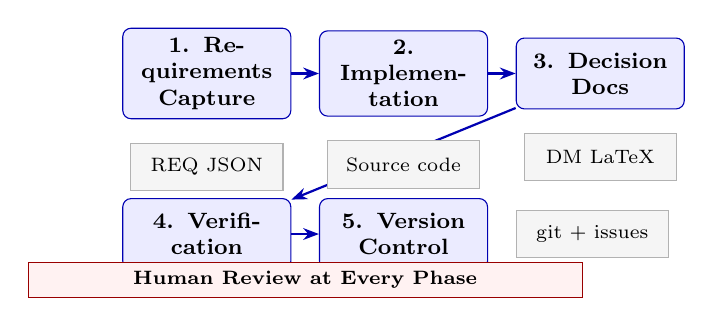
\begin{tikzpicture}[
    phase/.style={
        rectangle, rounded corners=3pt, draw=blue!70!black,
        fill=blue!8, text width=1.9cm, minimum height=0.9cm,
        align=center, font=\footnotesize\bfseries
    },
    artifact/.style={
        rectangle, draw=gray!60, fill=gray!8,
        text width=1.7cm, align=center,
        font=\scriptsize, minimum height=0.6cm
    },
    arr/.style={-{Stealth[length=2mm]}, thick, blue!70!black},
    labelstyle/.style={font=\scriptsize\itshape, text=gray!70!black}
]
% Phases in a flow
\node[phase] (p1) {1. Requirements\\Capture};
\node[phase, right=0.35cm of p1] (p2) {2. Implemen-\\tation};
\node[phase, right=0.35cm of p2] (p3) {3. Decision\\Docs};
\node[phase, below=1.0cm of p1] (p4) {4. Verifi-\\cation};
\node[phase, right=0.35cm of p4] (p5) {5. Version\\Control};

% Arrows between phases
\draw[arr] (p1) -- (p2);
\draw[arr] (p2) -- (p3);
\draw[arr] (p3) -- (p4);
\draw[arr] (p4) -- (p5);

% Artifacts
\node[artifact, below=0.3cm of p1] (a1) {REQ JSON};
\node[artifact, below=0.3cm of p2] (a2) {Source code};
\node[artifact, below=0.3cm of p3] (a3) {DM LaTeX};
\node[artifact, right=0.35cm of p5] (a5) {git + issues};

% Human review bar
\node[rectangle, draw=red!60!black, fill=red!5,
      text width=6.8cm, align=center, font=\scriptsize\bfseries,
      minimum height=0.45cm, below=0.35cm of $(p4)!0.5!(p5)$]
      (review) {Human Review at Every Phase};

\end{tikzpicture}
\caption{Five-phase methodology for AI-assisted compliance development. Human review occurs at every phase transition.}
\label{fig:methodology}
\end{figure}

\subsection{Phase 1: Requirements Capture}

Government projects begin with requirements derived from applicable standards. In our methodology, the developer identifies the governing standards (e.g., NIST SP 800-132 for key derivation) and instructs the Claude Code agent to generate a structured requirements document.

The agent produces requirements in machine-readable JSON format, enabling downstream tooling to generate formatted documents and traceability matrices. Each requirement includes:

\begin{itemize}[leftmargin=*]
    \item A unique identifier (e.g., \texttt{REQ-1.1})
    \item The governing standard and section reference
    \item The requirement text
    \item Classification as mandatory or recommended
    \item Verification method (inspection, test, analysis)
\end{itemize}

Listing~\ref{lst:req-json} shows an excerpt from the SendCUIEmail requirements document, generated with Claude Code assistance and reviewed by the developer.

\begin{lstlisting}[style=json, caption={Requirements specification excerpt (REQ-2026-001)}, label={lst:req-json}]
{
  "id": "REQ-1.1",
  "standard": "FIPS 197",
  "section": "Section 1",
  "text": "The tool SHALL use the Advanced
    Encryption Standard (AES) algorithm
    for all file encryption operations.",
  "priority": "mandatory",
  "verification": "inspection"
}
\end{lstlisting}

Requirement text uses RFC~2119 \cite{rfc2119} keywords (SHALL, SHOULD, MAY) to distinguish mandatory from recommended requirements, following the convention established in IETF and NIST publications. The developer's role shifts from \textit{authoring} requirements to \textit{reviewing} them---verifying that the AI's interpretation of the standard is correct and that no requirements are omitted. This review-centric workflow is faster than drafting from scratch while preserving the technical judgment that compliance demands.

\subsection{Phase 2: Implementation with Compliance Awareness}

During implementation, the Claude Code agent operates within the project's \texttt{CLAUDE.md} context, which encodes the compliance standards and architectural constraints. The \texttt{AGENTS.md} file (used in the SendCUIEmail project) provides persistent instructions that survive across sessions, as shown in Listing~\ref{lst:agentsmd}:

\begin{lstlisting}[style=powershell, caption={AGENTS.md compliance context excerpt}, label={lst:agentsmd}]
## Compliance Standards

- **FIPS 140-2**: AES-256-CBC encryption
- **NIST SP 800-132**: PBKDF2-HMAC-SHA256
    key derivation (100,000 iterations)
- **NIST SP 800-171**: CUI handling
- **32 CFR Part 2002**: CUI marking
\end{lstlisting}

This ensures that every agent session begins with awareness of the applicable standards, reducing the risk of non-compliant suggestions.

\subsection{Phase 3: Decision Documentation}

Government compliance frequently requires documenting \textit{why} a particular approach was chosen, not merely \textit{what} was implemented. Decision memoranda serve this purpose. In our methodology, when the developer makes a design choice (e.g., selecting Cinzel over Trajan Bold for CUI headers, or choosing TikZ over PDF manipulation for form layout), they instruct the agent to generate a formal decision memo.

The LaTeX/Decisions repository implements a template-wrapper pattern where each decision memo defines metadata variables and content, then includes a shared template:

\begin{lstlisting}[style=powershell, caption={Decision memo template pattern}, label={lst:dm-pattern}]
\newcommand{\UniqueID}{DM-2026-002}
\newcommand{\DocumentDate}{January 19, 2026}
\newcommand{\AuthorName}{PDF Tools Working Group}
\newcommand{\SubjectField}{Font Selection for
    CUI Header Text}
\newcommand{\dmContent}{...}
\input{_template.tex}
\end{lstlisting}

This pattern enables the AI agent to produce new decision memos by following the established template, ensuring consistency across the documentation package.

\subsection{Phase 4: Verification}

The final phase produces verification documents that map each requirement to its implementation evidence. The agent reads the source code, locates the relevant implementation for each requirement, and generates a verification matrix with file paths, line numbers, and explanatory text.

Table~\ref{tab:verification-excerpt} shows an excerpt from the SendCUIEmail verification document.

\begin{table}[htbp]
\centering
\caption{Verification matrix excerpt (VER-2026-001)}
\label{tab:verification-excerpt}
\begin{tabularx}{\columnwidth}{lXl}
\toprule
\textbf{Req.} & \textbf{Evidence} & \textbf{Method} \\
\midrule
REQ-1.1 & \texttt{Encrypt.ps1}: \texttt{[Aes]::Create()} call & Inspection \\
REQ-1.2 & \texttt{\$KEY\_SIZE = 32} (256 bits) & Inspection \\
REQ-2.3 & \texttt{\$ITERATIONS = 100000} & Inspection \\
REQ-3.1 & {\small\texttt{RandomNumberGenerator}} usage & Inspection \\
\bottomrule
\end{tabularx}
\end{table}

\subsection{Phase 5: Version Control and Interaction Traceability}
\label{sec:methodology-git}

The preceding development phases produce artifacts, but compliance also demands \textit{evidence of process}---a verifiable record of who made which decisions, when changes were introduced, and how human-agent interactions shaped the final deliverables. We use git version control and GitHub issues as complementary traceability mechanisms.

\subsubsection{Git as Audit Trail}

Every meaningful action---creating a requirements document, fixing a review finding, adding a compliance scan---is captured as an atomic git commit on the project's main branch. Each commit message describes the compliance-relevant change (e.g., ``Fix all 13 review findings from issue~\#1; add QA standards framework''). This produces a linear, tamper-evident history that auditors can inspect with standard tooling (\texttt{git log}, \texttt{git diff}).

Git's properties align directly with government configuration management requirements. NIST SP 800-53 CM-3 (Configuration Change Control) requires organizations to ``document, approve, and track changes to the system'' \cite{nist80053}. The git commit log serves as this change record: each commit is cryptographically hashed, timestamped, attributed to an author, and linked to its parent commits. Unlike informal change logs, git history cannot be silently altered without breaking the hash chain.

The project uses Semantic Versioning (SemVer) with a \texttt{CHANGELOG.md} following the Keep a Changelog convention. Version numbers encode the significance of changes: major versions for structural reorganization, minor versions for new content, and patch versions for corrections. Each release is tagged (\texttt{git tag~-a~vX.Y.Z}) and the changelog entries reference the GitHub issues that motivated each change. This provides a human-readable change history that complements the machine-level detail in the git log.

The Security Verification Toolkit case study (Section~\ref{sec:casestudy-toolkit}) embeds the git commit hash directly into its compliance attestation PDFs, binding each attestation to a specific, reproducible configuration state.

\subsubsection{GitHub Issues as Interaction Log}

While git captures \textit{what changed}, GitHub issues capture \textit{why it changed} and \textit{who directed the change}. All human-agent interactions in this project are logged as GitHub issues using a structured labeling scheme:

\begin{itemize}[leftmargin=*]
    \item \texttt{human-prompt}: A human directive to the AI agent (e.g., ``expand agents.json with additional agent roles'')
    \item \texttt{agent-output}: Agent-generated analysis or findings (e.g., ``13 review findings per IEEE 1028 inspection'')
    \item \texttt{decision}: A design or process decision with rationale (e.g., ``IT security standards are standard review criteria'')
\end{itemize}

This labeling scheme creates a queryable audit record. An auditor can filter by \texttt{human-prompt} to see every directive the human issued, by \texttt{agent-output} to see every AI-generated analysis, or by \texttt{decision} to trace the rationale for each design choice. The combination provides bidirectional traceability between human intent and AI action---a key requirement when demonstrating human-in-the-loop oversight to government auditors.

All five agents in the multi-agent configuration (Section~\ref{sec:agents}) include interaction logging in their system prompts, requiring them to create GitHub issues for every substantive human-agent exchange. This ensures that the audit trail is comprehensive regardless of which agent is active.

% ============================================================
\section{Case Study: SendCUIEmail}
\label{sec:casestudy-sendcui}

\subsection{Project Overview}

SendCUIEmail is a PowerShell-based tool for encrypting files before email transmission, designed for environments where Public Key Infrastructure (PKI) or S/MIME certificate exchange is impractical. The tool addresses a common gap in federal and contractor environments: the need to transmit CUI securely when the only available channel is unencrypted email.

The project's compliance scope spans six federal standards and regulations:

\begin{enumerate}[leftmargin=*]
    \item \textbf{FIPS 197} \cite{fips197}: AES algorithm specification
    \item \textbf{FIPS 140-2} \cite{fips1402}: Cryptographic module validation
    \item \textbf{NIST SP 800-132} \cite{nist800132}: Password-based key derivation
    \item \textbf{NIST SP 800-38A} \cite{nist80038a}: Block cipher modes of operation
    \item \textbf{NIST SP 800-90A} \cite{nist80090a}: Random number generation
    \item \textbf{32 CFR Part 2002} \cite{32cfr2002}: CUI marking and handling
\end{enumerate}

\subsection{AI-Assisted Artifacts}

Over the course of development, Claude Code assisted in producing the following compliance artifacts:

\subsubsection{Requirements Document (REQ-2026-001)}

A JSON-formatted requirements specification containing 29 requirements across six categories: encryption algorithm, key derivation, random number generation, password handling, file format, and platform requirements. The JSON source-of-truth enables automated generation of formatted PDF documents via a Python build script.

\subsubsection{Decision Memoranda (DM-2026-001 through DM-2026-007)}

Seven formal decision memos documenting design choices:

\begin{itemize}[leftmargin=*]
    \item \textbf{DM-001}: Cross-platform support strategy
    \item \textbf{DM-002}: File size limit rationale (10~MB)
    \item \textbf{DM-003}: Password transmission method (out-of-band per NIST SP 800-63B \cite{nist80063b})
    \item \textbf{DM-004}: Verification document numbering scheme
    \item \textbf{DM-005}: Multi-category CUI support per 32~CFR~2002.20(a)(3)
    \item \textbf{DM-006}: Beta readiness assessment
    \item \textbf{DM-007}: Recipient instruction format selection (HTML)
\end{itemize}

\subsubsection{Verification Document (VER-2026-001)}

A line-by-line code verification mapping all 29 requirements to specific implementation evidence in the source code, including file paths, function names, and configuration values.

\subsection{Cryptographic Implementation}

The core encryption implementation demonstrates how AI-assisted development can produce compliant code. The encrypted file format is:

\begin{multline}
\text{Output} = \text{Salt}_{128} \| \text{IV}_{128} \| {} \\
\text{AES-256-CBC}(K, \text{IV}, \text{Plaintext})
\end{multline}

where $K$ is derived via PBKDF2-HMAC-SHA256:

\begin{equation}
K = \text{PBKDF2}(\text{password}, \text{Salt}, 100000, 256)
\end{equation}

The implementation uses exclusively platform-provided cryptographic libraries (\texttt{System.Security.Cryptography}), avoiding third-party dependencies that would complicate FIPS validation. When Windows FIPS mode is enabled, the tool leverages CMVP-validated cryptographic modules (e.g., Certificate \#4515, Kernel Mode Cryptographic Primitives Library, validated under FIPS 140-2 on Windows 10; specific certificate numbers vary by Windows version).

\subsection{Recipient Experience Design}

A significant AI-assisted design contribution was the recipient decryption workflow. The tool generates a self-contained HTML instruction document (\texttt{Decrypt\_Instructions.html}) with an embedded PowerShell one-liner:

\begin{lstlisting}[style=powershell, caption={Decryption logic (simplified from production code)}, label={lst:oneliner}]
$f=Read-Host "File"
$p=Read-Host "Password"
$d=[IO.File]::ReadAllBytes($f)
$k=[Rfc2898DeriveBytes]::new(
    $p,$d[0..15],100000,"SHA256")
$a=[Aes]::Create()
$a.Key=$k.GetBytes(32)
$a.IV=$d[16..31]
$c=$a.CreateDecryptor()
    .TransformFinalBlock($d,32,$d.Length-32)
[IO.File]::WriteAllBytes(
    ($f-replace'\.Locked$',''),$c)
\end{lstlisting}

This design requires no software installation by recipients---only PowerShell, which is built into every modern Windows installation. The production code uses \texttt{SecureString} with \texttt{SecureStringToBSTR} conversion and file picker dialogs; the listing above is a functionally correct simplification using plaintext password input for clarity. The AI agent helped iterate on the production one-liner to minimize its length while maintaining compliance with the cryptographic parameter requirements.

% ============================================================
\section{Case Study: Decision Documentation System}
\label{sec:casestudy-decisions}

The LaTeX/Decisions repository demonstrates AI-assisted creation of a reusable documentation system for formal decision memoranda. Government programs frequently require Decision Memoranda (DMs) to document technical and policy choices with traceable rationale.

\subsection{Template Architecture}

The system uses a template-wrapper pattern where a shared base template (\texttt{\_template.tex}) defines the document layout---headers with organizational logo, footers with document ID and page numbering, and standardized section formatting---while individual decision documents supply metadata and content through LaTeX command definitions.

This separation of concerns enables AI agents to produce new decision memos by populating the established template structure, ensuring visual and structural consistency without requiring the agent to understand the full LaTeX layout implementation.

\subsection{SF901 CUI Coversheet Compliance}

Three decision memos (DM-2026-001 through DM-2026-003) document the technical approach to generating Standard Form~901 CUI coversheets:

\begin{enumerate}[leftmargin=*]
    \item \textbf{Implementation approach}: LaTeX template recreation rather than PDF manipulation, chosen for alignment with existing infrastructure and independence from external tools.
    \item \textbf{Font selection}: Cinzel (open-source, SIL OFL) chosen over Trajan Bold (commercial) for the CUI header, balancing visual fidelity with licensing constraints.
    \item \textbf{Layout strategy}: TikZ with absolute positioning for pixel-precise form reproduction, justified by the form's stability (unchanged since November 2018 per GSA records).
\end{enumerate}

Each decision memo follows the format required by many government programs: identification of options considered, evaluation criteria, selected approach, and rationale with regulatory references.

% ============================================================
\section{Case Study: Security Verification Toolkit}
\label{sec:casestudy-toolkit}

The third case study examines the Security Verification Toolkit \cite{nist80053}, a pure-Bash security scanning and compliance documentation system that automates the verification of federal security controls. Unlike SendCUIEmail (which implements a single compliance function) or the Decision Documentation System (which manages process artifacts), the toolkit addresses the \textit{continuous compliance verification} challenge: demonstrating ongoing adherence to NIST SP 800-53 and NIST SP 800-171 controls through automated scanning and attestation generation.

\subsection{Scope and Standards}

The toolkit implements 14 NIST SP 800-53 controls and 11 NIST SP 800-171 controls across eight security control families, with each scan mapped to its governing control in machine-readable JSON. The standards addressed include:

\begin{itemize}[leftmargin=*]
    \item \textbf{NIST SP 800-53} \cite{nist80053}: RA-5 (Vulnerability Scanning), CM-6 (Configuration Settings), CM-8 (Component Inventory), SA-11 (Developer Testing), SI-2/3/4/5/12 (Information Integrity), SC-8 (Transmission Protection), MP-6 (Media Sanitization), CA-2 (Assessment)
    \item \textbf{NIST SP 800-171} \cite{nist800171}: 11 corresponding CUI protection requirements
    \item \textbf{NIST SP 800-88} \cite{nist80088}: Media sanitization (secure deletion)
    \item \textbf{BOD 22-01} \cite{bod2201}: CISA Known Exploited Vulnerabilities cross-referencing
    \item \textbf{FIPS 199} \cite{fips199}: Security categorization of federal information
\end{itemize}

\subsection{Requirements Traceability}

The toolkit maintains a complete traceability chain in JSON format:

\begin{equation*}
\text{Requirement} \rightarrow \text{NIST Control} \rightarrow \text{Script} \rightarrow \text{Test} \rightarrow \text{Evidence}
\end{equation*}

A \texttt{mapping.json} file links 14 functional requirements (FR-001 through FR-014) to NIST controls, implementation scripts, and test cases, navigable in three directions: by script, by NIST 800-53 control, and by NIST 800-171 control. This bidirectional traceability enables auditors to verify compliance from any starting point---a requirement that many government programs mandate but few tools automate.

The AI agent assisted in generating this traceability framework, producing the initial JSON mappings from the NIST control catalog and iterating with the developer to ensure completeness. The machine-readable format enables downstream automation: generating formatted traceability reports, validating that no requirements are orphaned, and detecting when code changes break previously-verified controls.

\subsection{Automated Attestation Generation}

A distinguishing feature of the toolkit is its automated generation of formal compliance attestations as PDFs via LaTeX templates. After each scan run, the system produces timestamped, checksummed attestation documents suitable for inclusion in government compliance packages. Each attestation includes:

\begin{itemize}[leftmargin=*]
    \item Toolkit version and git commit hash (configuration management)
    \item Scan timestamp in ISO 8601 UTC
    \item SHA-256 checksums of all scan outputs
    \item NIST control mappings for each finding
    \item CUI markings where applicable
\end{itemize}

The toolkit's design philosophy---\textit{``You are only as good as your last scan''}---enforces that every scan run overwrites previous results, preventing stale attestations from being presented as current evidence. This maps directly to the continuous monitoring requirements of NIST CA-7.

\subsection{Multi-Agent Development}

The toolkit itself was developed using a multi-agent architecture with defined roles: Lead Systems Engineer, QA Engineer, Windows Developer, Documentation Engineer, and Lead Software Developer. Agent coordination uses GitHub issues as the communication channel---the same interaction logging pattern adopted in this paper's methodology. This represents a mature implementation of the multi-agent compliance workflow described in Section~\ref{sec:agents}, validated across 2.7 major versions and over 140 GitHub issues.

% ============================================================
\section{Multi-Agent Workflow}
\label{sec:agents}

Claude Code's \texttt{--agents} mode enables orchestrated workflows where multiple specialized agents collaborate on a project. For government compliance work, we propose the role-based agent architecture shown in Figure~\ref{fig:agents}.

\begin{figure}[htbp]
\centering
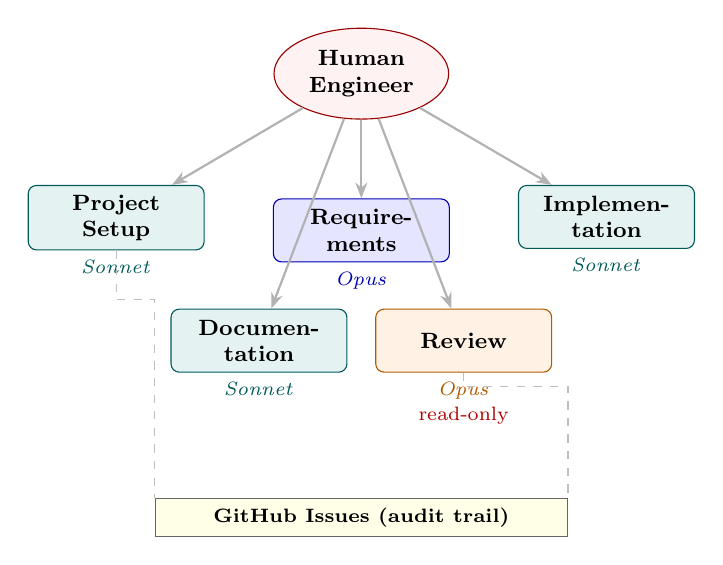
\begin{tikzpicture}[
    agent/.style={
        rectangle, rounded corners=3pt, draw=#1!70!black,
        fill=#1!10, text width=2.0cm, minimum height=0.8cm,
        align=center, font=\footnotesize\bfseries
    },
    model/.style={
        font=\scriptsize, text=#1!70!black
    },
    tools/.style={
        rectangle, draw=gray!50, fill=gray!5,
        font=\scriptsize, align=center, minimum height=0.4cm
    },
    arr/.style={-{Stealth[length=2mm]}, thick, gray!60},
    human/.style={
        ellipse, draw=red!60!black, fill=red!5,
        font=\footnotesize\bfseries, align=center,
        minimum width=2.0cm, minimum height=0.7cm
    }
]

% Human at top
\node[human] (human) {Human\\Engineer};

% Agents row 1
\node[agent=teal, below left=1.0cm and 1.2cm of human] (setup) {Project\\Setup};
\node[agent=blue, below=1.0cm of human] (req) {Require-\\ments};
\node[agent=teal, below right=1.0cm and 1.2cm of human] (impl) {Implemen-\\tation};

% Agents row 2
\node[agent=teal, below=2.4cm of human, xshift=-1.3cm] (doc) {Documen-\\tation};
\node[agent=orange, below=2.4cm of human, xshift=1.3cm] (rev) {Review};

% Model labels
\node[model=teal, below=0pt of setup] {\textit{Sonnet}};
\node[model=blue, below=0pt of req] {\textit{Opus}};
\node[model=teal, below=0pt of impl] {\textit{Sonnet}};
\node[model=teal, below=0pt of doc] {\textit{Sonnet}};
\node[model=orange, below=0pt of rev] {\textit{Opus}};

% No-write indicator
\node[font=\scriptsize\color{red!70!black}, below=9pt of rev] {read-only};

% Arrows from human
\draw[arr] (human) -- (setup);
\draw[arr] (human) -- (req);
\draw[arr] (human) -- (impl);
\draw[arr] (human) -- (doc);
\draw[arr] (human) -- (rev);

% GitHub issues bar
\node[rectangle, draw=black!60, fill=yellow!10,
      text width=5.0cm, align=center,
      font=\scriptsize\bfseries, minimum height=0.4cm,
      below=2.0cm of $(doc)!0.5!(rev)$]
      (gh) {GitHub Issues (audit trail)};

% Dashed lines to GitHub
\draw[dashed, gray!50] (setup.south) -- ++(0,-0.62) -| (gh.north west);
\draw[dashed, gray!50] (rev.south) -- ++(0,-0.17) -| (gh.north east);

\end{tikzpicture}
\caption{Multi-agent architecture for compliance projects. Teal agents use Sonnet; blue/orange agents use Opus. The review agent has read-only access (NIST SP 800-53 AC-5). All agents log interactions to GitHub issues.}
\label{fig:agents}
\end{figure}

\subsection{Agent Roles}

\begin{enumerate}[leftmargin=*]
    \item \textbf{Project Setup Agent}: Initializes repository structure, creates \texttt{CLAUDE.md} with compliance context, establishes documentation templates and directory layout.
    \item \textbf{Requirements Agent}: Analyzes governing standards and generates structured requirements documents in JSON format.
    \item \textbf{Implementation Agent}: Writes compliant code within the constraints defined by the requirements and \texttt{CLAUDE.md} context.
    \item \textbf{Documentation Agent}: Produces decision memoranda, verification documents, and traceability matrices.
    \item \textbf{Review Agent}: Audits artifacts for completeness, citation accuracy, and cross-reference integrity.
\end{enumerate}

\subsection{Agent Configuration}

Agent definitions are stored in a JSON configuration file that specifies each agent's role, model selection, permitted tools, and a detailed system prompt encoding compliance context. Table~\ref{tab:agent-config} summarizes the five-agent configuration developed for this paper.

\begin{table*}[htbp]
\centering
\caption{Agent configuration summary (agents.json)}
\label{tab:agent-config}
\begin{tabularx}{\textwidth}{llllX}
\toprule
\textbf{Agent} & \textbf{Model} & \textbf{Phase} & \textbf{QA Standard} & \textbf{Key Capability} \\
\midrule
project-setup & Sonnet & Setup & --- & Repo structure, build config, templates \\
requirements & Opus & Phase 1 & IEEE 29148 & Standard interpretation, JSON requirements \\
implementation & Sonnet & Phase 2 & --- & Compliant code within REQ constraints \\
documentation & Sonnet & Phase 3 & MIL-STD-498 & Decision memos, verification docs, LaTeX \\
review & Opus & Phase 4 & IEEE 1028, NIST 800-53 AC-5 & Audit with no write access (read-only) \\
\bottomrule
\end{tabularx}
\end{table*}

Model selection reflects the cognitive demands of each role: the \texttt{requirements} and \texttt{review} agents use Opus for its stronger reasoning over regulatory interpretation and cross-reference validation, while \texttt{implementation} and \texttt{documentation} use Sonnet for its favorable speed-to-quality ratio on structured, template-following tasks. Notably, the \texttt{review} agent is denied write and edit tools, enforcing a separation-of-duties principle where auditors identify problems but do not fix them.

\subsection{Workflow Orchestration}

The multi-agent workflow proceeds through the five phases described in Section~\ref{sec:methodology}, with each agent operating within its defined scope. The key advantage of this architecture is \textit{context isolation}: the requirements agent does not need the full implementation context, and the documentation agent can focus on artifact generation without the overhead of the full codebase in its context window.

This isolation is particularly valuable for government projects where compliance documentation can be extensive---a full NIST SP 800-171 assessment may reference over 100 security requirements, and maintaining all of these in a single agent context is impractical. The separation-of-duties between the \texttt{documentation} and \texttt{review} agents also mirrors the organizational controls common in government programs, where the author of a compliance artifact should not be the sole reviewer.

% ============================================================
\section{Discussion}
\label{sec:discussion}

\subsection{Quality of AI-Generated Compliance Artifacts}

Our experience indicates that Claude Code produces compliance artifacts that are \textit{structurally sound} but require careful human review for \textit{substantive accuracy}. The AI reliably generates:

\begin{itemize}[leftmargin=*]
    \item Correct document structure and formatting
    \item Appropriate standard references (e.g., citing NIST SP 800-132 for PBKDF2)
    \item Reasonable requirement decomposition
    \item Accurate code-to-requirement tracing when given source access
\end{itemize}

Areas requiring human review include:

\begin{itemize}[leftmargin=*]
    \item \textit{Regulatory interpretation}: Whether a requirement is ``mandatory'' vs. ``recommended'' per the governing standard
    \item \textit{Completeness}: Whether all applicable requirements from a standard have been captured
    \item \textit{Citation precision}: Verifying specific section numbers within standards
    \item \textit{Organizational context}: Tailoring requirements to the specific compliance posture of the organization
\end{itemize}

\subsection{The Review-Centric Workflow}

The most significant shift introduced by AI-assisted compliance development is the transition from an \textit{authoring} model to a \textit{review} model. In traditional compliance work, an engineer reads the governing standard, interprets its requirements, drafts the compliance artifact, and submits it for review. With AI assistance, the engineer specifies the standard and reviews the AI-generated artifact for accuracy.

This shift has two implications. First, it is faster: reviewing a draft is consistently less effort than producing one from scratch. Second, it changes the \textit{skill profile} required: the engineer must be a competent reviewer of compliance documents rather than a competent author. This is a meaningful distinction---many engineers who understand the technical standards struggle with the formal writing conventions of government documentation.

\subsection{Human-in-the-Loop Compliance}

Government frameworks increasingly require evidence of human oversight in automated processes. Claude Code's permission model---where each file write, command execution, and code edit requires explicit developer approval---provides natural evidence of human-in-the-loop oversight. Every action taken by the agent is logged and approved, creating an audit trail that maps to the ``authorized use'' requirements common in government security frameworks.

The \texttt{CLAUDE.md} convention further supports compliance by encoding organizational and project-specific constraints that persist across sessions. An organization's compliance officer could define \texttt{CLAUDE.md} templates that encode mandatory requirements, ensuring that all AI-assisted development within the organization operates within approved boundaries.

\subsection{Standards-Based Review Process}

The review agent itself operates according to established QA standards, making the review process auditable and reproducible. Table~\ref{tab:qa-standards} maps each aspect of the review process to its governing standard.

\begin{table*}[htbp]
\centering
\caption{QA standards applied to the AI-assisted review process}
\label{tab:qa-standards}
\begin{tabularx}{\textwidth}{llX}
\toprule
\textbf{Standard} & \textbf{Control} & \textbf{Application} \\
\midrule
IEEE 1028 \cite{ieee1028} & Software Reviews & Review structure: severity classification (CRITICAL/MINOR), findings format, disposition \\
IEEE 29148 \cite{ieee29148} & Requirements Engineering & Traceability verification: standard $\rightarrow$ requirement $\rightarrow$ implementation $\rightarrow$ test \\
NIST SP 800-53 \cite{nist80053} & AC-5: Separation of Duties & Review agent denied write/edit tools; auditors cannot modify what they audit \\
NIST SP 800-53 \cite{nist80053} & SA-11: Developer Testing & Claims verified against source files; assertions checked against implementation \\
ISO/IEC 25010 \cite{iso25010} & Software Quality & Documentation quality: completeness, accuracy, consistency checks \\
MIL-STD-498 \cite{milstd498} & A.5.19: Traceability & Cross-reference integrity between REQ, VER, DM, and source code \\
\bottomrule
\end{tabularx}
\end{table*}

This standards-based approach ensures that the review process itself can withstand audit scrutiny---a critical consideration for government programs where the QA methodology must be as defensible as the artifacts it evaluates. All review findings are documented as GitHub issues with structured severity, recommendation, and standard-violated fields, providing a traceable audit record per IEEE~1028.

\subsection{Limitations}

Several limitations should be noted:

\begin{enumerate}[leftmargin=*]
    \item \textbf{Model knowledge currency}: LLM training data has a cutoff date, meaning recent revisions to standards (e.g., updates to NIST SP 800-171 Rev.~3, or the transition from FIPS 140-2 to FIPS 140-3 for new CMVP submissions since 2021) may not be reflected. Developers must verify that AI-cited standards are current.
    \item \textbf{No formal verification}: AI-generated compliance claims are assertions, not proofs. They do not substitute for formal testing, independent audit, or certification processes such as CMVP validation.
    \item \textbf{Organizational specificity}: Government compliance is highly context-dependent. The same standard may be interpreted differently across agencies, and AI agents lack organizational knowledge without explicit instruction.
    \item \textbf{Classification boundaries}: AI tools operating in cloud-connected modes are unsuitable for classified work. The methodology presented here applies only to unclassified and CUI environments.
\end{enumerate}

\subsection{Reproducibility and Process Documentation}

This paper itself was produced using the methodology it describes. The white paper repository maintains a two-tier documentation structure: \texttt{PROCESS.md} provides a human-readable executive summary of each development session, while GitHub issues serve as the authoritative, machine-queryable record of all human-agent interactions.

As of this writing, the repository contains 14 GitHub issues spanning 6 development sessions, with each issue labeled according to the scheme described in Section~\ref{sec:methodology-git}. The git history contains 9 semantically versioned commits (v0.1.0 through v0.5.0, with ongoing work toward v0.6.0), each corresponding to a distinct compliance-relevant action. Together, these records provide sufficient information for an independent team to reproduce the development process or for an auditor to verify that every artifact has a documented provenance chain.

This dual-track approach---git for configuration management, GitHub issues for interaction traceability---mirrors the separation between configuration management (NIST SP 800-53 CM-3) and audit logging (NIST SP 800-53 AU-3) that government frameworks prescribe. The combination ensures that the process is documented at both the artifact level (what changed) and the decision level (why it changed).

% ============================================================
\section{Future Work}
\label{sec:future}

Several directions merit further investigation:

\begin{enumerate}[leftmargin=*]
    \item \textbf{Automated compliance testing}: Integrating AI agents with continuous integration pipelines to validate compliance assertions against code changes.
    \item \textbf{Standard-specific agents}: Training or fine-tuning agents on specific government standards (e.g., a NIST SP 800-171 specialist agent) to improve requirement extraction accuracy.
    \item \textbf{Cross-reference validation}: Building tools that automatically verify citations between compliance artifacts (requirements $\leftrightarrow$ verification $\leftrightarrow$ code).
    \item \textbf{FedRAMP and CMMC application}: Extending the methodology to broader compliance frameworks such as FedRAMP authorization packages and CMMC assessments.
    \item \textbf{Comparative studies}: Quantitative comparison of AI-assisted vs. manual compliance documentation effort across multiple projects and team sizes.
\end{enumerate}

% ============================================================
\section{Conclusion}
\label{sec:conclusion}

This paper has demonstrated a methodology for applying AI-assisted development tools---specifically Claude Code---to the challenge of building software that meets government compliance requirements. Through three case studies, we showed that AI agents can produce structurally sound compliance artifacts including requirements specifications, decision memoranda, verification documents, and automated compliance attestations, while the interactive approval model provides the human oversight that government frameworks require.

The key insight is not that AI replaces compliance expertise, but that it \textit{restructures} the compliance workflow. The engineer's role shifts from author to reviewer, the documentation burden decreases without sacrificing rigor, and the multi-agent architecture enables scalable compliance workflows for projects of varying complexity.

As government agencies and contractors face increasing pressure to demonstrate compliance across expanding regulatory frameworks, AI-assisted tooling offers a practical path to maintaining documentation quality without proportional increases in engineering effort. The methodology, agent configurations, and process documentation presented here provide a foundation for teams seeking to adopt this approach.

% ============================================================
\section*{Acknowledgments}

This paper and its supporting artifacts were developed using Claude Code (Anthropic, model: Claude Opus). The development process itself serves as a case study for the methodology presented. All source materials, including the white paper LaTeX source, agent configurations, and process documentation, are available at \url{https://github.com/brucedombrowski/WhitePaper}.

% ============================================================
\bibliographystyle{ieeetr}
\bibliography{references}

\end{document}
